\documentclass[review, 3p, authoryear]{elsarticle}
%\documentclass[twocolumn]{article}
\usepackage{graphicx}
\usepackage{lineno}
\usepackage{hyperref}
\usepackage{xspace}

\title{SEXTANTE, a versatile open--source  library for spatial data analysis}
\author[uni]{Olaya, V.\corref{cor1}}
\cortext[cor1]{Corresponding author. Email:\texttt{volaya@unex.es}}
\ead{volaya@unex.es}

\author[uni]{Gim\'enez, J. C.}
\address[uni]{Universidad de Extremadura. Campus de Plasencia. Avda. Virgen del Puerto 2. 10600, C\'aceres, Spain. Tlf. (+34)927427000}


\date{\today}

\begin{document}

\linenumbers

\begin{frontmatter}

\begin{abstract}
This article presents the SEXTANTE library, an open--source spatial data analysis library which leverages the access to a comprehensive (300+) set of algorithms and spatial operations, along with additional components to maximize its productivity and ease of use. Special emphasis has been put on the correct design of the core of the library, in order to maximize its versatility and make it easier for both developers and end users to implement and use algorithms. Its architecture makes it very simple to reuse algorithms and incorporate them in any software, and thus expands the reach of spatial data analysis beyond its traditional place in desktop GIS and related tools. Applications currently using SEXTANTE as their spatial data analysis provider include desktop GIS, business intelligence tools and Web Processing Service (WPS) servers, among others.

\end{abstract}
\begin{keyword}
SEXTANTE \sep Spatial data analysis \sep Geoprocessing \sep WPS
\end{keyword}

\end{frontmatter}

\section{Introduction}

Spatial data analysis is a key component of Geographical Information Systems and has been integrated in GIS tools since their origins. However, geographical information is nowadays more popular than ever and spatial data analysis can be applied in many different contexts outside a classical GIS software. 

Although the current context is appropriate for expanding spatial analysis into new fields and target it to new groups of users, using spatial analysis algorithms is usually restricted to GIS or scientific applications. Also, most of them are deeply embedded within the application's architecture, making it hard to reuse them from a different software. Certain applications might be used in a library--like fashion (i.e. applications with a command--line interface which can be called from other programs acting as frontends), but a fully satisfying solution is yet to be developed, since all the current ones do not have the right features needed to be able to supply spatial data analysis capabilities and be seamlessly integrated in other kinds of software. Architecture and design problems are a common issue, specially interoperability issues related to the communication between the application providing spatial data analysis algorithms and the one consuming them. This is usually solved with filesystem--based solutions, which are far from being an optimal solution, as they limit the flexibility of the operations and might also cause performance issues.

The development of a flexible and versatile spatial data analysis library would, therefore, help to provide a powerful platform to incorporate spatial analysis in a wide range of applications, from classical desktop GISs to others that previously did not incorporate this kind of analysis tools. 

Desktop GISs are the main type of software for which a spatial data analysis library has special interest. Most desktop GISs feature spatial data analysis capabilities to some extent, usually as an intrinsic part of the software, but sometimes provided by third--party libraries. Even desktop GIS with a large array of geoalgorithms might rely on external programs, specially on open--source ones. 

This kind of reusability of algorithms should be the main aim of a spatial data analysis library. The number of projects and applications that integrate spatial analysis capabilities from other different software is large, which indicates there is a need for such a library and also an important group of potential users of it among desktop applications. Examples of this will be given in the next section.

An important number of geographical data viewers have appeared in the last years, becoming increasingly popular, specially 3D ones (globes). These viewers have also become an important tool in the scientific community, and when expanded with analysis capabilities they provide a useful tool for scientific tasks \citep{kisilevich_geo-spade_2010, di_martino_integratinggoogle_2009}. A flexible spatial data analysis library will notably reduce the time needed to integrate geoalgorithms in such viewers.

Web GIS applications have recently started to incorporate analytical capabilities, in which is one of the main trends of the so--called GeoWeb \citep{voloder_future_2010}. This will turn Web Mapping into Web GIS, where not only visualization of spatial data is implemented in a Web application, but all the other functionalities of a full GIS as well. Web--based clients are used to access remote processing services \citep{wolf_web-client_2009}, while desktop GIS can also access those services if they incorporate built--in client functionalities. This creates a need for Web servers capable of serving not just spatial data, but also processes. The WPS OGC standard has been developed to standardize the definition and access to such services. 

WPS server development has been centered around the service itself, but not much effort has been put into adding geoalgorithms to be served, so they are currently of limited utility from a general point of view. \citet{Diaz2008FOSS4G} and \citet{Bergenheim2009GRASS} exposed several algorithms for hydrological analysis and line generalization, respectively, through a WPS service. However, these, as many other examples, are not general solutions but rather particular cases applied to a given field. They involve a fair amount of programming and configuration to get from the algorithm working locally to the one being served through a WPS service. Additional effort is needed to expose the algorithm, while, ideally, it should automatically integrate itself into the server just like it integrates into the desktop application.

GRASS algorithms have been used in similar works by \citet{yue_geopw:_2009} and \citet{li_sharing_2009}, among others. The latest, however, mentions the difficulties that arise due to the different data formats used by the GIS and the server, and the need to implement a filesystem--based solution to allow communication between them. A direct implementation of geoalgorithms in the server, based on a common data model, is a recommended alternative.

The application of grid computing techniques has been considered as one of the most relevant advantages of a remote spatial data processing network \citep{padberg_gridification_2009}, since it could solve storage and computing issues in such fields as the analysis of Digital Elevation Models, which usually implies massive amounts of data \citep{lanig_towards_2008}. Thus, integration in a grid computing scenario might be considered in the design of a spatial data analysis library and its algorithms.

Finally, non--GIS applications are as relevant as GIS ones in the current context, since geographical information has become a fundamental part of many disciplines and sectors. Addressing the needs of these applications has been a key concern in the development of the SEXTANTE library. 

Among these applications, spatial ETL (Extract, Transform, Load) tools play an important role. A spatial ETL incorporates spatial data into data integration software \citep{coudert_spatial_2008}, combining both spatial and non--spatial data. Geoalgorithms can be incorporated as a part of the transformation component of the ETL tool, providing analysis capabilities along with common operations such as coordinate system conversion, usually present in this kind of applications.  %A well--defined semantic is needed to incorporate geoalgorithms in a generic fashion into spatial ETL's.

Although the integration of spatial analysis in this kind of tools is recent, \citet{Marr_interoperablegis} already pointed out the necessity of combining spatial analysis algorithms and modeling software, and discussed interoperability of both data and models as the key element to achieve a correct integration.



\section{Related work}\label{relatedWork}
%
%Within the scope of this article, the following categories are of interest to justify the necessity of a library such as the one presented here, as well as to explain the possible relations between it and other software projects. This last circumstance is specially relevant considering the open--source philosophy adopted.
%
%\begin{itemize}
%	\item Existing spatial data analysis software. These will provide ideas to define the architecture and main components, as well as geoalgorithms that can be ported. Usage of these software by other applications should be studied to define the best way to implement an integration mechanism for our library. 
%	
%	Ancillary libraries that might be be reused to build the core components will be reviewed as well. Libraries for common tasks not directly related to spatial data, such as logging, will not be included here since they are not relevant for the aim of this article. 
%	\item Targeted software. Software packages featuring some kind of extension mechanism that allows to include third--party geoalgorithms as a part of their capabilities. These are potential users of the library, and should shape its main characteristics and capabilities. 
%\end{itemize}

%\subsection{Existing spatial data analysis software}

The number of different tools related to spatial data analysis is large in both open--source and proprietary software.  \citet{Smith2010GA} listed  nearly 200 software packages with GIS and spatial data analysis features.

Many small projects exist which just cover a given subfield of spatial analysis, most of them originating in the scientific community. Well--known examples of such software are FRAGSTATS \citep{McGarigal2002FRAGSTATS}, for spatial pattern analysis; CrimeStat \citep{Levine2010Crimestat}, for crime statistic analysis or gstat \citep{pebesma_gstat:_1998}, for multivariable geostatistical modeling, prediction and simulation. These applications are a good source of algorithms and analysis concepts, but their design as analysis platforms is not robust enough for a more generic usage.


Generic collections of geoalgorithms are found mostly on desktop GIS. Open--source solutions are particularly rich in this area, with many of them focusing on analysis above other common capabilities of GIS applications such as the creation of cartography. GRASS \citep{neteler2007openSourceGIS}, SAGA \citep{Conrad2007phd} or ILWIS are all good representatives of this kind of applications. Among proprietary software, whether commercial or not, there are also several packages with advanced spatial analysis tools. ArcGIS, Idrisi or PCRaster, all contain large collections of algorithms covering most areas of spatial analysis. 

Although different in their features, most of these software packages have a similar design of their analytical capabilities. In most cases, algorithms and core functionalities can be accessed through an Application Program Interface (API), so they can be scripted and called from a regular programming language. The development of new geoalgorithms is also done this way, since core functionality is also exposed. In the case of open--source applications, development can be done in the same manner as it was with already existing algorithms, since the code of the core classes is available.

For the purpose of developing a spatial data analysis library, ArcGIS, SAGA and GRASS are the most interesting, since their design is closer to what is needed for such a library. In both SAGA and GRASS, algorithms contain the implementation of the analytical process, along with a precise description of the parameters needed to run the algorithm, but user--interface elements do not have to be added by the programmer. The description of parameters is later used to provide interaction methods to the user. Command--line syntax is defined based on them, and so are the GUI elements and windows. In the case of SAGA, the SAGA GUI application is directly responsible for that, while in the case of GRASS this is done by any of the available frontends.

If a description of both inputs and outputs of the process is given, ArcGIS scripts can be turned into toolbox elements, which might be regarded as an equivalent of a SAGA module or a GRASS command. This allows the script to be executed in other tools within ArcGIS such as the ModelBuilder.

The existence of a well--defined semantic appears to be a fundamental element to create a generic platform for implementing and using geoalgorithms, as it is a common element of the ones mentioned above.

Although it does not contain a large set of algorithms, the PySAL \citep{Rey2007PySAL} library shares a common aim with the SEXTANTE library presented in this article, and it is the only other open--source independent library currently available for spatial data analysis.

The R system for statistical computing \citep{R2010}, although not a GIS, contains spatial data analysis routines. It can be extended by creating new ``packages'', several of which deal with spatial data, both raster and vector.

The Java Topology Suite (JTS) library has become a de facto standard for handling geometries in the Java GIS world, as it is used by many of its main projects like GeoTools, OpenJUMP or uDiG. The need for a common ground to be defined in a spatial data analysis library for data handling makes JTS a natural choice for this task.

Integration between many of the software packages above is rather common, as it was already pointed out, evidencing that algorithms can be consumed not just by direct users, but also by external applications to expand their capabilities.

A good example of this is the RSAGA package \citep{Brenning2008SAGA}. RSAGA integrates the R computing language with the command--line version of SAGA, including a set of R commands that allow to call SAGA algorithms from within the R environment. Reverse integration between GRASS and R (that is, using R from GRASS) has also been developed \citep{Bivand200Geocomp} 

Gstat and IDRISI are another good example of that. Gstat can be accessed from within IDRISI, which already contains a large set of built--in geoalgorithms.


%\subsection{Targeted software}

\section{The SEXTANTE library}

All the above circumstances justify the development of a spatial data analysis library and outline the main features that would be desirable to find in it. In order to maximize its utility and effectiveness, such a library should have the following characteristics:

\begin{itemize}
	\item Easy implementation of geoalgorithms. Ideally, a spatial data analysis algorithm should only contain the code needed to perform the calculations that constitute the core of the algorithm itself. This way, anyone capable of writing down some mathematical ideas working with spatial data should be also capable of implementing the algorithm in the library, which will expose it to users of all the applications using it. Knowledge of geospatial data analysis methods is encouraged over GIS or computer--related skills, giving the opportunity of implementing their algorithms to researchers who work with spatial data but may lack the necessary skills to deal with more advanced issues, mainly those related with GIS architectural elements.
	\item Comprehensiveness. It should cover the main types of analysis operations and be able to work with the most common types of data. This should include, but not be limited to, raster and vector data in both 2D and 3D, as well as images as a particular kind of raster data.
	\item Delegation of data handling. All data handling tasks should be performed by the underlying software, which will supply the data to the library and its algorithms in a transparent manner. This will allow the library to run on any system which is capable of handling spatial data, regardless of its format or origin. The library should be able to ``understand'' the data objects of the application on top of which it is running, but not the primary sources of those data objects. This way, different sources (i.e. vector data from a shapefile, from a database connection or from a WFS service) will be handled in a similar manner, transparently.  This also has a significant effect in making algorithm development easier and more straightforward, since developers do not have to worry about data handling issues, but just 
about consuming and producing spatial data.	
	
	Delegation of data handling is the main lack of existent spatial data analysis software, and, consequently, constitutes the main difference and improvement of the library presented in this article.
	\item Ability to reuse existing geoalgorithms. The large body of spatial data analysis algorithms implemented in other libraries and applications cannot be ignored when creating this library. Mechanisms for wrapping those algorithms should be implemented so they can be exposed through the library. Algorithms served via remote services should be considered as well.
	\item Open source. Distribution under an open--source license will facilitate the integration of the library in any software without legal restrictions.

\end{itemize}

The SEXTANTE library has been developed with the aim of constituting a platform that addresses the previous needs and can be of utility for the applications and usages described in Section \ref{relatedWork}. To do this, and to meet the requirements stated above, SEXTANTE has an architecture comprised of the following parts:

\begin{itemize}
	\item A set of base classes upon which geoalgorithms can be easily developed. 
	\item Data bindings to connect the library with the data objects used by the application consuming its geoprocessing capabilities. These bindings wrap the application's data object so they can be accessed by SEXTANTE. 
	\item A comprehensive set of geoalgorithms. Currently more than 300 algorithms are part of the library. They are divided in the following groups (the number of algorithms in each group is indicated between brackets): tools for point layers (20), raster layer analysis (9), basic hydrological analysis (10), topology (4), tools for line layers (15), vegetation indices (10), statistical methods (10), rasterization and interpolation (9), raster creation tools (7), location/allocation (2), raster categories analysis (11), buffers (6), tools for polygon layers (16), 3D (4), basic tools for raster layers (23), pattern analysis (5), cost, distances and routes (15), visibility and lighting (10), local statistics (16), table tools (3), TIN (5), geostatistical analysis of raster layers (3), tools for vector layers (32), image processing (16), indices and other hydrological parameters (15), vectorization (5), focal statistics (14), fire modeling (2), profiles (4), fuzzy logic (2), geomorphometry and terrain analysis (11), reclassify raster layers (6) and calculus tools for raster layers (20). 
\end{itemize}

Among the base classes, the most important one is the \emph{Geoalgorithm} class, which is the one to extend when creating a new geoalgorithm. Creating an algorithm is done by overriding two methods, namely \emph{describeAlgorithm} and \emph{processAlgorithm}. These are used, respectively, to describe the inputs and outputs of the algorithm, and to process the input data and generate outputs. That is, to define the semantic of the algorithm and to implement the algorithm itself. The rules to define the semantic are heavily inspired by the ones in SAGA, adding new types of outputs (text strings, graphics and individual numerical values) and inputs (3D layers) to have a more versatile range of data objects that can be used or produced by an algorithm. This is also similar to what can be found in other software packages like GRASS or ArcGIS, since they have many points in common as it was already mentioned.

Bindings wrap spatial data objects from the application running SEXTANTE and create objects that can be understood by SEXTANTE algorithms. Creation of new layers or tabular data is also done through the corresponding binding classes, which communicate with the application and delegate the task of creating them. Since creation of data is not done directly by SEXTANTE, but instead by the application, this allows to output results in as many different ways as the application supports. 

Much like the mentioned example of an algorithm taking a vector layer as input, if an algorithm produces an output vector layer, this can be saved to the filesystem (in as many formats as the application is capable of writing it), added to a database, uploaded to a remote server through a WFS--T service or even streamed through any available stream. An interface named \emph{IOutputChannel} has been defined for this matter. An output channel can be understood as the element that defines what to do with data objects generated by the algorithm. 

Once again, the developer of a geoalgorithm does not have to deal with these issues. Available channels depend on the current data bindings being used and then selection of a channel is done when executing the algorithm. The developer just produces the output but does not define how it is handled or where it is stored.

Further information about programming SEXTANTE algorithms can be found in \citet{Olaya2011Programming}

Along with the core of the library,  a set of graphical components have been developed to access the algorithms provided by SEXTANTE. These elements make it easier to incorporate SEXTANTE--based analysis capabilities into an application such as a desktop GIS, and provide a common interface for running SEXTANTE algorithms across different programs. 

Four are the graphical elements of SEXTANTE:

\begin{itemize}
	\item The \emph{Toolbox} (Figure \ref{Fig:Toolbox}), which represents the main graphical element of SEXTANTE. Most users will employ only this element in a normal session. From its window, algorithms can be run as single processes, and also as batch processes, executing the corresponding algorithm on a set of input data files.

\begin{figure}[!hbt]
 \centering
 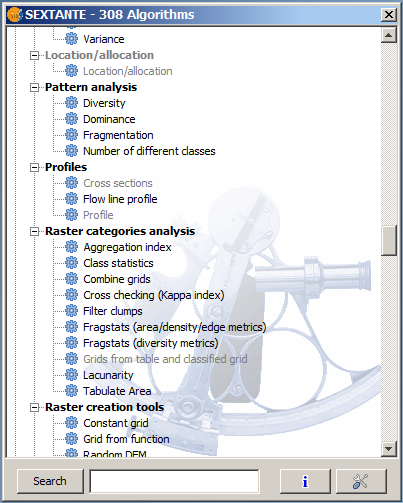
\includegraphics[width=.5\columnwidth]{toolbox.png}
\caption{SEXTANTE toolbox}
\label{Fig:Toolbox}
\end{figure}

	\item The \emph{Graphical Modeler} (Figure \ref{Fig:Modeler}). The modeler can be used to define a global process that involves several single processes, each of them consisting of a geoalgorithm. Relations between those processes can be defined so the input of one of them can be the output of a previous one, thus setting a workflow. All this is done through an intuitive interface.
	
	
\begin{figure*}[!hbt]
 \centering
 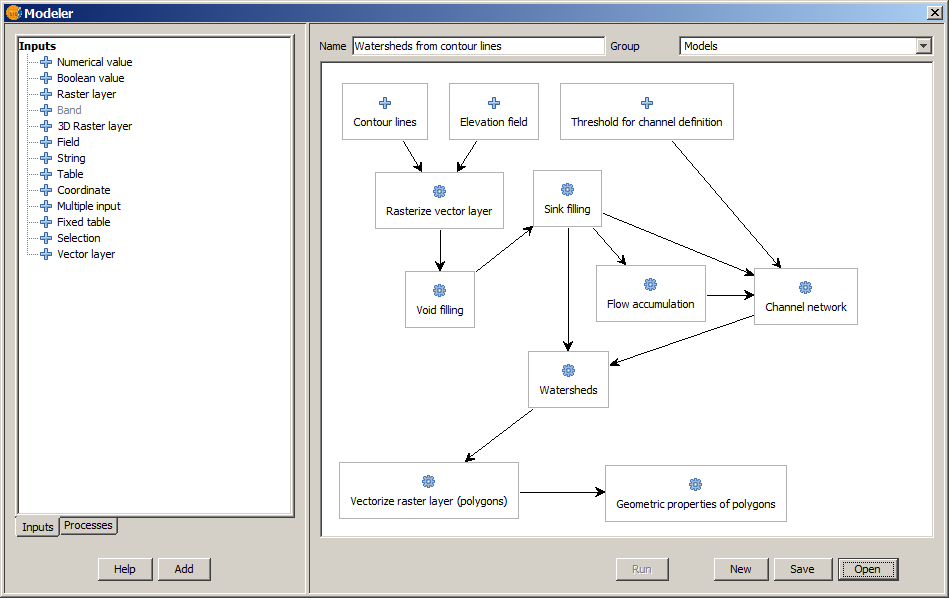
\includegraphics[width=.85\textwidth]{modeller.png}
\caption{SEXTANTE graphical modeler}
\label{Fig:Modeler}
\end{figure*}

	\item The \emph{Command Line Interface}. A built--in command line for advanced users, which gives more flexibility and allows for the creation of small scripts. 
	\item The \emph{Command History Manager}. Whenever a SEXTANTE algorithm is run, a new element is added to the SEXTANTE history. Using this element, the command history can be browsed and certain actions can be repeated, just double clicking on a single command or selecting a block of them.

\end{itemize}

Graphical components link SEXTANTE algorithms with the application's interface and add some interaction between them. Bindings for the graphical part of the application running SEXTANTE are also needed, which perform tasks such as adding output results to a map view in the application or retrieving the extent of that view to be used as the analysis region for an algorithm.

All this architecture is summarized in Figure \ref{Fig:Architecture}, which clearly shows the independence of SEXTANTE algorithms from the software consuming them, both in terms of data and GUI. 

\begin{figure}[!hbt]
 \centering
 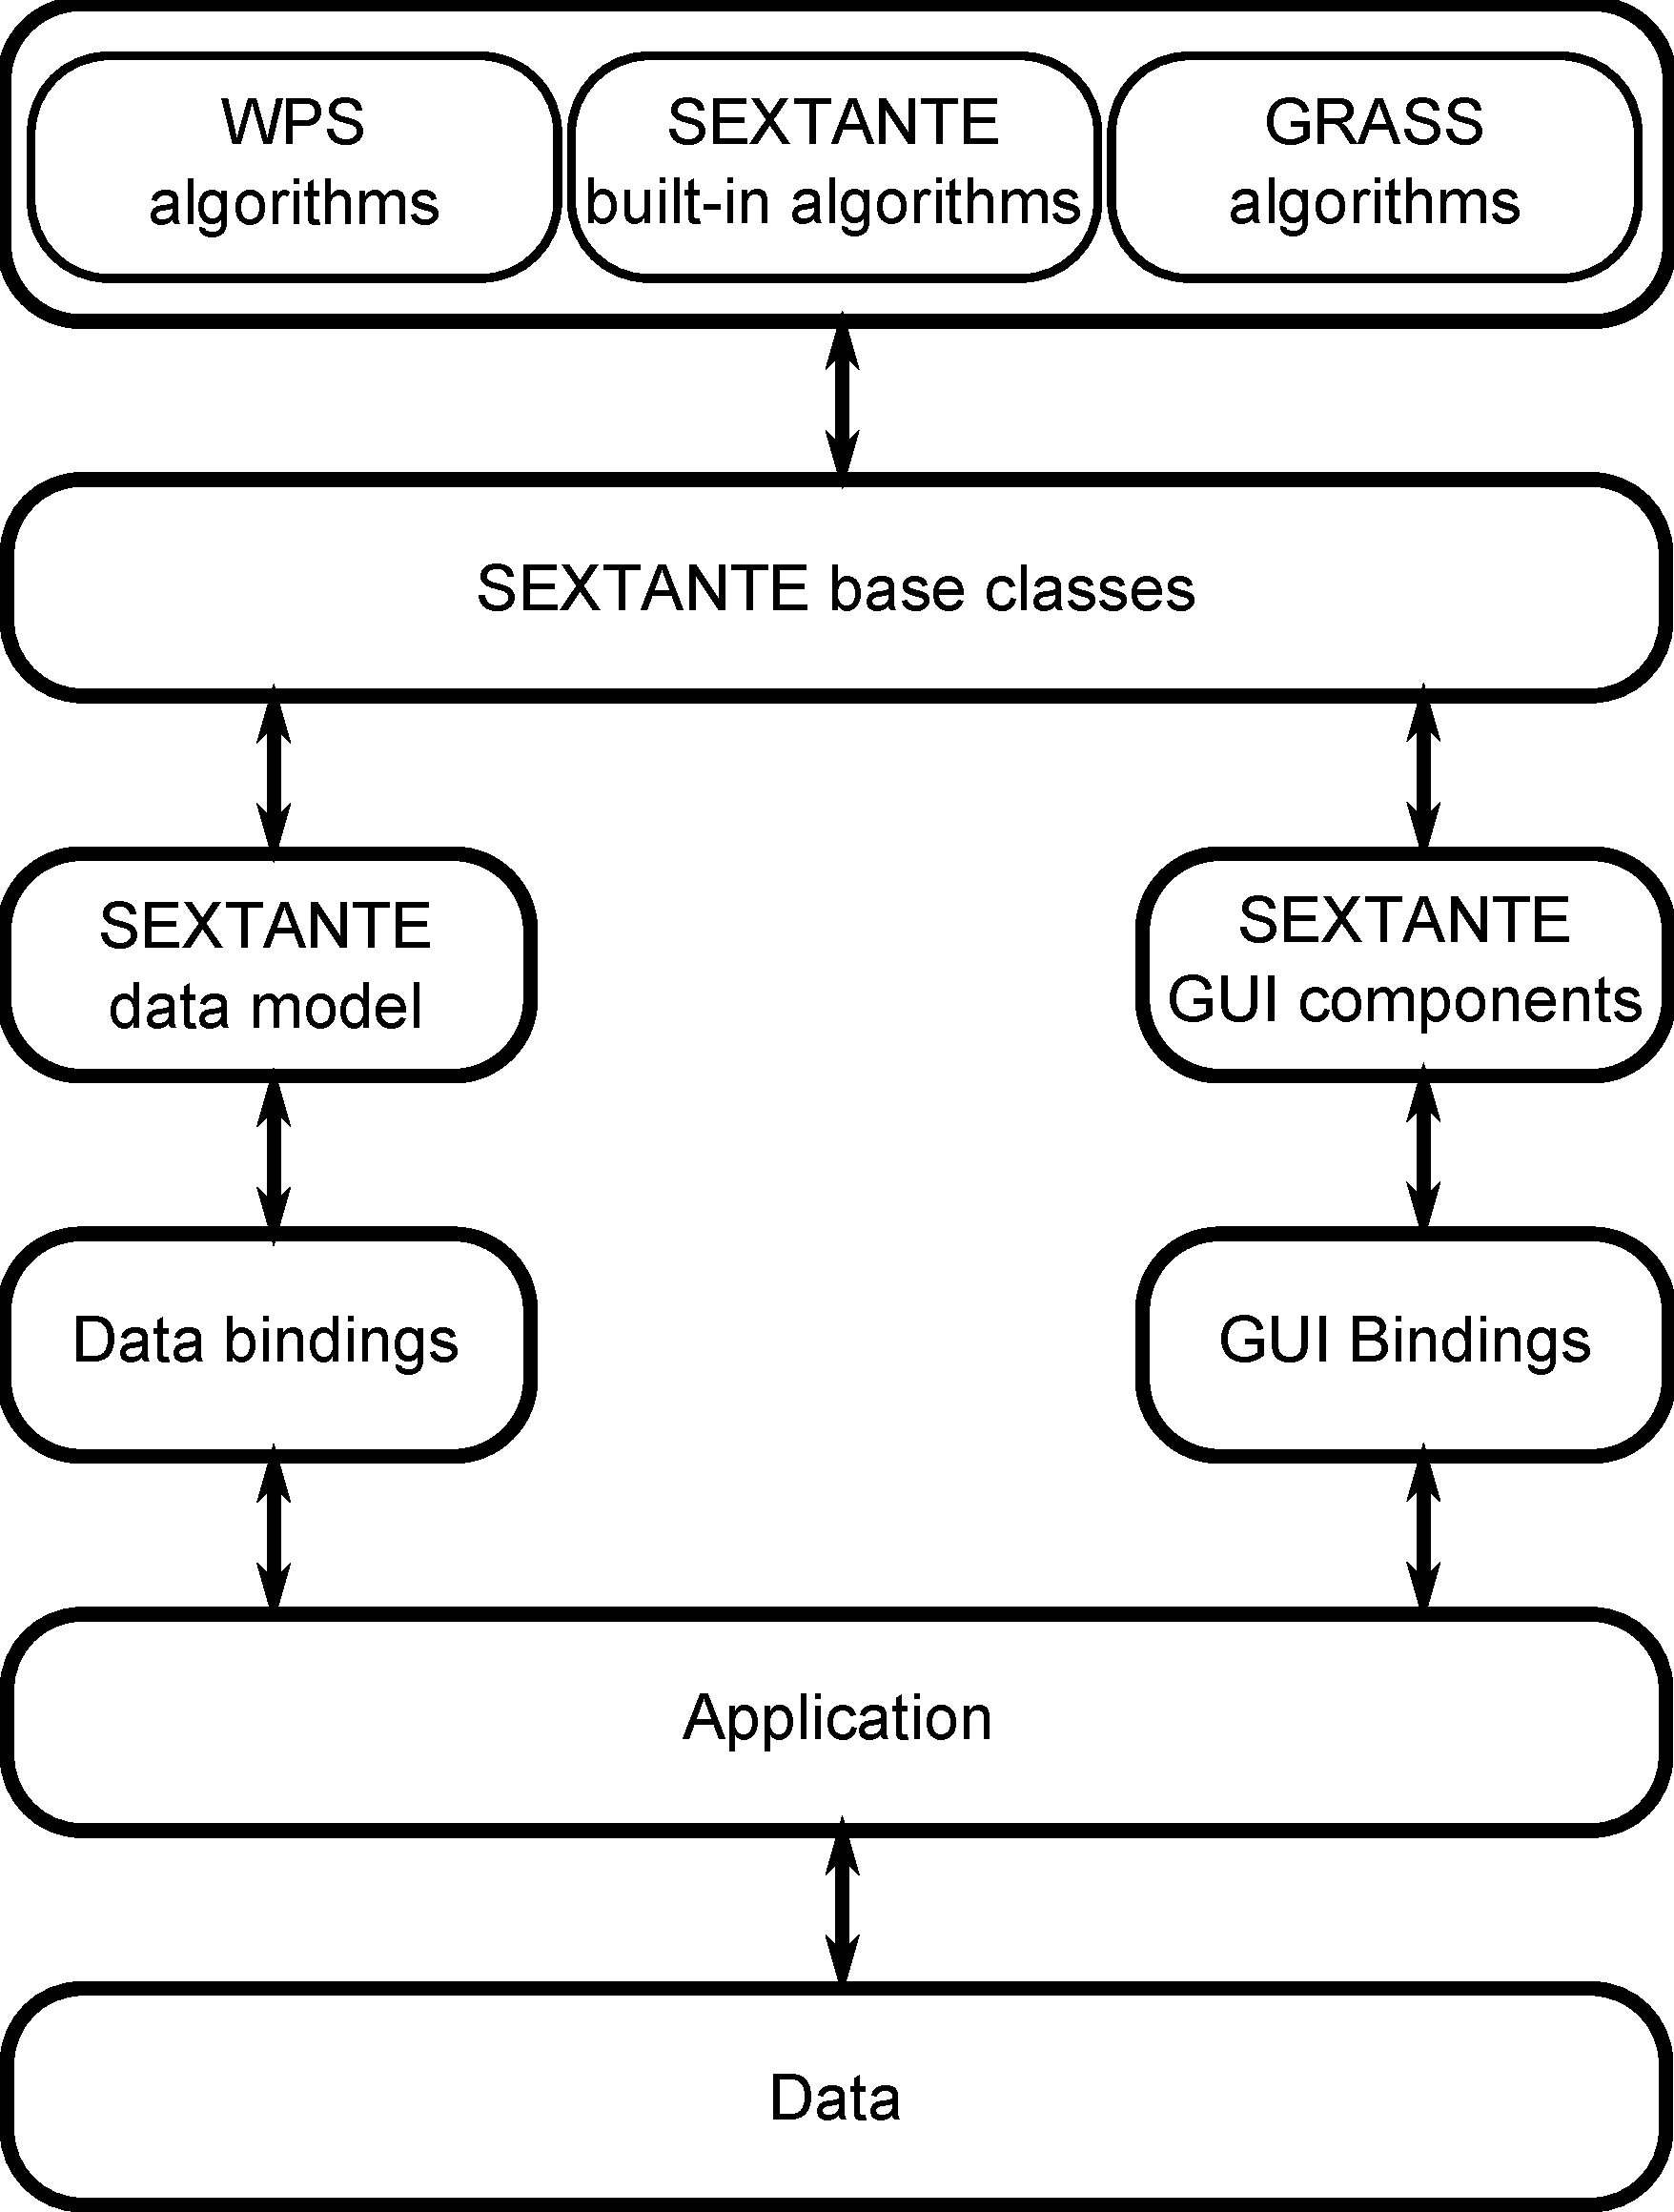
\includegraphics[width=.5\columnwidth]{architecture.pdf}
\caption{Architecture of the SEXTANTE library}
\label{Fig:Architecture}
\end{figure}

It also shows how the set of built--in algorithms can be expanded by wrapping external algorithms. Wrappers for GRASS algorithms and remote WPS processes are currently available as part of the latest version of SEXTANTE. A wrapper for the R statistical computing language is currently being developed by the SEXTANTE development team along with a working group from the University of Castell\'on (Spain)


\section{Current usage}

SEXTANTE is currently implemented as part of several applications, all of them open--source. In the desktop GIS category, OpenJUMP\footnote{http://www.openjump.org/index.html} and gvSIG\footnote{http://gvsig.org} rely on SEXTANTE for their analytical capabilities and include it in their latest versions. In the case of gvSIG, additional tools have been added by the development team to further enhance the integration of both applications. Although gvSIG already contains	its own set of geoprocessing tools, these are also included as part of SEXTANTE or are in the process of being ported, so eventually all spatial analysis in gvSIG will be performed through SEXTANTE.

BeETLe \citep{Martinez2010Beetle} is a software project that extends Kettle, a ETL part of the Pentaho business intelligence suite, to include spatial data elements. SEXTANTE is used to provide spatial analysis routines. In a similar manner, Spatial Data Integrator \citep{coudert_spatial_2008} extends Talend, a data integration software, adding spatial data I/O, as well as SEXTANTE--based geolgorithms. 

The 52North WPS server includes SEXTANTE since its 2.0 RC3 version. Previous to that integration, \citet{granell_service-oriented_2010} successfully combined a subset of SEXTANTE algorithms with an older version of this server and exposed them as WPS services. The 52North WPS server has also been used to test the WPS client in SEXTANTE. A ``clean'' copy of SEXTANTE (that is, just the core classes but without any geoalgorithm) was used to access a 52North WPS server with the full set of SEXTANTE algorithms. This replicated the functionality of a local copy of SEXTANTE, but with all geoalgorithms being obtained as remote services.

Current developments being carried on by the SEXTANTE development team or third parties include bindings with ArcGIS and Glob3, a framework for 3D GIS based on NASA's World Wind globe.


\section{Limitations and further work}

Although special care has been taken to correctly design the architecture of the library, it still presents some limitations and issues that need to be addressed. Also, some elements of the library are not fully developed or its functionality still can be improved. The following ones are the main weaknesses of SEXTANTE and constitute the areas in which further work should be done:

\begin{itemize}
	\item Topology. Support for topology is not considered in the current version of SEXTANTE. The data model used does not support topological information, although some algorithms related with topology exist, such as those aimed at correcting the topological structure of line and polygon layers. Most mainstream desktop GIS, as well as data libraries like the widely used GeoTools, do not support topology either, which makes it hard to develop a testbed for such functionalities. 
	\item 3D vector data. SEXTANTE uses the JTS library for handling geometries. Geometries in JTS are tridimensional (the JTS Coordinate class contains $x, y$ and $z$ components), but operations and additional elements are strictly bidimensional, and all of them ignore the $z$ component. Spatial indices, heavily used by many SEXTANTE algorithms, can only be applied in a planar context, so they are not suitable for 3D algorithms. Current 3D algorithms solve this issue using external additional libraries, but it would be desirable to have a fully--functional 3D library integrated in the core of SEXTANTE, providing the same capabilities as JTS does in 2D.
	\item Robust $vs$ flexible semantics. The semantic of a SEXTANTE geoalgorithm is not complete in many senses, which causes problems when linking it with other software in certain contexts. \citet{fernandoGGL} incorporated SEXTANTE into the GearScape Geoprocessing Language (GGL), a declarative language based on SQL92 which allows for the execution of complex geoalgorithms. Not all algorithms could, however, be included. Those that generate output results whose characteristics depend on the input layers are not suitable for this. For instance, an algorithm that generates a vector layer with an attributes table with a variable number of fields is not compatible with the semantic of GGL, since the number of fields cannot be known in advance but just at runtime.
	
	A more restrictive set of semantic rules could be implemented, but that would reduce the ease of developing a geoalgorithm and it would also be necessary to rewrite or remove some of the currently existing ones, since they would not fit into the new semantic context.
	 
\end{itemize}

Other limitations are beyond SEXTANTE itself. The main one is related to the handling of large raster datasets. Since SEXTANTE delegates all its data handling, a robust and capable platform is needed to incorporate such large datasets so they can be analyzed, and also to create such large ones when it is required by the algorithm. However, all the current Java GIS applications and libraries have some problems in this issue, which means that SEXTANTE algorithms cannot be applied with raster layers larger than a certain size, which is insufficient in many cases. Large vector datasets do not pose any problem, since several applications running SEXTANTE are capable of handling them and feature optimized routines specifically developed for that matter.

\section{Availability}

SEXTANTE can be downloaded from its official website\footnote{http://www.sextantegis.com}. Stable versions, as well as nightly builds, are available. Documentation for both users and developers is also freely available for download in editable and non--editable formats. Source code can be checked out anonymously from the SVN repository. Instructions are given in the SEXTANTE website.

SEXTANTE is distributed under a MIT license, while documents are distributed under a Creative Commons Attribution license

Applications using SEXTANTE are also available from different sources, and were mentioned in previous sections of this article.



\section{Conclusions}

The SEXTANTE library is a spatial data analysis library designed for maximum reusability and to provide a set of spatial analysis algorithms that meets the needs of most users. Providing an easy development of new algorithms has been one of the main concerns when designing its architecture, along with versatility in terms of data sources and outputs. The latter is accomplished by delegating data handling to the application running SEXTANTE, which makes algorithms independent from data sources in a transparent manner.

SEXTANTE is currently integrated in several applications. Many of this applications are desktop GIS, which also use the graphical components of SEXTANTE to allow for graphical user interaction.

\section{Acknowledgments}

The development of the SEXTANTE library has been founded by the Junta de Extremadura (local government of the Extremadura region, Spain), following its pioneering effort to support the development and use of open--source software in the public administration.

%\bibliography{biblio}{}
\bibliographystyle{apalike}

\begin{thebibliography}{}

\bibitem[Asociacion gvSIG, 2011]{webgvSIG}
Asociaci\'on gvSIG.
\newblock gvSIG Project official website.
\newblock \url{http://www.gvsig.org/web/}
\newblock Retrieved 13--February--2011.

\bibitem[Bergenheim et~al., 2009]{Bergenheim2009GRASS}
Bergenheim, W., Tiina, L., and Sarjakoski, T. (2009).
\newblock A web processing service for GRASS GIS to provide on-line
  generalisation.
\newblock In {\em Prooceedings of the 12th AGILE International Conference on
  Geographic Information Science 2009}.

\bibitem[Bivand, 2000]{Bivand200Geocomp}
Bivand, R. (2000).
\newblock Using the R statistical data analysis language on GRASS 5.0 GIS
  database files.
\newblock {\em Computers \& Geosciences}, 26:1043--1052.

\bibitem[Brenning, 2008]{Brenning2008SAGA}
Brenning, A. (2008).
\newblock {\em SAGA-Seconds Out (Hamburger Beitr�ge zur Physischen Geographie
  und Landschafts�kologie, vol. 19)}, chapter Statistical geocomputing
  combining R and SAGA: The example of landslide susceptibility analysis with
  generalized additive models, pages 23--32.

\bibitem[Conrad, 2007]{Conrad2007phd}
Conrad, O. (2007).
\newblock {\em SAGA - Entwurf, Funktionsumfang und Anwendung eines Systems f�r
  Automatisierte Geowissenschaftliche Analysen.}
\newblock PhD thesis, University of Goettingen.
\newblock \url{http://webdoc.sub.gwdg.de/diss/2007/conrad/conrad.pdf}.

\bibitem[Coudert, 2008]{coudert_spatial_2008}
Coudert, M. (2008).
\newblock Spatial Data Integrator - open source spatial {ETL}.
\newblock {\em {GEO:} connexion}, 7(2):56--57.

\bibitem[{De Smith} et~al., 2011]{Smith2010GA}
{de Smith}, M., Goodchild, M., and Longley, P. (2011).
\newblock {\em Geospatial Analysis (3rd edition). A Comprehensive Guide to
  Principles, Techniques and Software Tools}.

\bibitem[Diaz et~al., 2008]{Diaz2008FOSS4G}
Diaz, L., Granel, C., Gould, M., and Olaya, V. (2008).
\newblock An open service network for geospatial data processing.
\newblock In {\em Proceedings of the Free and Open Source Software for
  Geospatial (FOSS4G) Conference}.

\bibitem[Gonzalez and Leduc, 2010]{fernandoGGL}
Gonzalez, F. and Leduc, T. (2010).
\newblock GGL: A geo--processing definition language that enhance spatial sql
  with parameterization.
\newblock In {\em Proceedings of the 13th AGILE International Conference on
  Geographic Information Science 2010. Guimaraes, Portugal}.

\bibitem[Granell et~al., 2010]{granell_service-oriented_2010}
Granell, C., Diaz, L., and Gould, M. (2010).
\newblock Service-oriented applications for environmental models: Reusable
  geospatial services.
\newblock {\em Environmental Modelling and Software}, 25(2):182--198.

\bibitem[JPP, 2010]{JPP2010}
The Jump Pilot Project (JPP) (2010).
\newblock Open Jump official website.
\newblock \url{http://www.openjump.org/index.html}
\newblock Retrieved 13--February--2011.

\bibitem[Kisilevich et~al., 2010]{kisilevich_geo-spade_2010}
Kisilevich, S., Keim, D., and Rokach, L. (2010).
\newblock {GEO-SPADE} - a generic Google Earth-based framework for analyzing
  and exploring spatio-temporal data.
\newblock In {\em {ICEIS} 2010 - Proceedings of the 12th International
  Conference on Enterprise Information Systems}, volume 5 {HCI}, pages 13--20.

\bibitem[Lanig et~al., 2008]{lanig_towards_2008}
Lanig, S., Schilling, A., Stollberg, B., and Zipf, A. (2008).
\newblock {\em Towards standards-based processing of digital elevation models
  for grid computing through Web Processing Service {(WPS)}}, volume 5073
  {LNCS}.

\bibitem[Levine., 2010]{Levine2010Crimestat}
Levine., N. (2010).
\newblock {\em CrimeStat: A Spatial Statistics Program for the Analysis of
  Crime Incident Locations (v 3.3).}
\newblock {Ned Levine \& Associates, Houston, TX, and the National Institute of
  Justice, Washington, DC.}

\bibitem[Li et~al., 2009]{li_sharing_2009}
Li, X., Di, L., Han, W., Zhao, P., and Dadi, U. (2009).
\newblock Sharing and reuse of service-based geospatial processing through a
  web processing service.
\newblock In {\em 2009 17th International Conference on Geoinformatics,
  Geoinformatics 2009}.

\bibitem[Marr et~al., 1997]{Marr_interoperablegis}
Marr, A., Pascoe, R., and Benwell, G. (1997).
\newblock Interoperable GIS and spatial process.
\newblock In {\em Proceedings of Second Annual Conference of GeoComputation �97
  \& SIRC �97}.

\bibitem[Martinez and Simonazzi., 2010]{Martinez2010Beetle}
Martinez, C. and Simonazzi., W. (2010).
\newblock Proyecto beetle: acercando SEXTANTE al mundo ETL.
\newblock In {\em Proceeding of the IV Jornadas de SIG Libre. Girona, Spain.
  March 10-12}.

\bibitem[Martino et~al., 2009]{di_martino_integratinggoogle_2009}
Martino, S.~D., Bimonte, S., Bertolotto, M., and Ferrucci, F. (2009).
\newblock {\em Integrating Google Earth within OLAP tools for multidimensional
  exploration and analysis of spatial data}, volume 24 {LNBIP}.

\bibitem[McGarigal et~al., 2002]{McGarigal2002FRAGSTATS}
McGarigal, K., Cushman, S.~A., Neel, M.~C., and Ene., E. (2002).
\newblock {\em FRAGSTATS: Spatial Pattern Analysis Program for Categorical
  Maps}.
\newblock University of Massachusetts, Amherst, Amherst.
\newblock \url{www.umass.edu/landeco/research/fragstats/fragstats.html}.

\bibitem[Neteler and Mitasova, 2007]{neteler2007openSourceGIS}
Neteler, M. and Mitasova, H. (2007).
\newblock {\em Open {S}ource {GIS}: {A} {GRASS} {GIS} {A}pproach}.
\newblock Springer, New York, third edition.

\bibitem[Olaya, 2011]{Olaya2011Programming}
Olaya, V. (2011).
\newblock {\em SEXTANTE programming guide}.

\bibitem[Padberg and Greve, 2009]{padberg_gridification_2009}
Padberg, A. and Greve, K. (2009).
\newblock Gridification of {OGC} web services: Challenges and potential.
\newblock {\em {GIS-Zeitschrift} fur Geoinformatik}, (3):77--81.

\bibitem[Pebesma and Wesseling, 1998]{pebesma_gstat:_1998}
Pebesma, E. and Wesseling, C. (1998).
\newblock Gstat: A program for geostatistical modelling, prediction and
  simulation.
\newblock {\em Computers and Geosciences}, 24(1):17--31.

\bibitem[{R Development Core Team}, 2010]{R2010}
{R Development Core Team} (2010).
\newblock {\em R: A Language and Environment for Statistical Computing}.
\newblock Vienna, Austria.
\newblock {ISBN} 3-900051-07-0.

\bibitem[SEXTANTE Development Team, 2011]{SEXTANTE2011}
SEXTANTE development team. 
\newblock SEXTANTE Project official website.
\newblock \url{http://www.sextantegis.com}. 
\newblock Retrieved 13--February--2011.

\bibitem[Rey and Anselin, 2007]{Rey2007PySAL}
Rey, S. and Anselin, L. (2007).
\newblock Pysal: A python library of spatial analytical methods.
\newblock {\em The Review of Regional Studies}, 37:5--27.

\bibitem[Voloder, 2010]{voloder_future_2010}
Voloder, I. (2010).
\newblock Future progress of the geoweb.
\newblock In {\em {MIPRO} 2010 - 33rd International Convention on Information
  and Communication Technology, Electronics and Microelectronics, Proceedings},
  pages 1309--1315.

\bibitem[Wolf and Howe, 2009]{wolf_web-client_2009}
Wolf, E. and Howe, K. (2009).
\newblock Web-client based distributed generalization and geoprocessing.
\newblock In {\em Proceedings of the International Conference on Advanced
  Geographic Information Systems and Web Services, {GEOWS} 2009}, pages
  123--128.

\bibitem[Yue et~al., 2009]{yue_geopw:_2009}
Yue, P., Gong, J., Di, L., Yuan, J., Sun, L., and Wang, Q. (2009).
\newblock {\em {GeoPW:} Towards the geospatial processing Web}, volume 5886
  {LNCS}.

\end{thebibliography}



\end{document}